\chapter{Introduction}
\epigraph{``It has not escaped our notice that the specific pairing we have postulated immediately suggests a possible copying mechanism for the genetic material."}{Watson and Crick, Nature \cite{watson1953}}

``Structure is function'' is an often heard mandate in structural biology. In 1962, the Nobel Prize in medicine was awarded to Crick, Watson and Wilkins for discovering the double helix structure of DNA. The detailed knowledge of a biological macromolecules's structure, including the 3D arrangement of its atoms, is the first step in understanding its function and hence, biological mechanisms.

Since then, hundreds of thousands of macromolecular structures have been solved. The popular method of choice to solve macromolecular structures for several decades has been X-ray crystallography, in which the diffraction patterns of X-rays scattered from a crystallized protein are used to deduce its structure. Crystallization is required to amplify the weak signal, that is, the diffraction pattern of a single molecule. A large, perfectly ordered crystal can produce a diffraction pattern that is resolvable to a sufficiently high resolution to allow 3D reconstruction. However, a serious limitation to X-ray crystallography is that many proteins and viruses are resistant to crystallization, thereby limiting the ability to study these macromolecules. Enter single particle cryo-electron microscopy (cryo-EM). Although cryo-EM was first introduced as early as the 1970's, it has grown into a ``revolution'' resisting crystallization \cite{Kuhlbrandt1443} since 2013, with its rapid advancement in leaps and bounds. Cryo-EM allows the study of macromolecules in vivo, in their functionally active state, unlike X-ray crystallography, in which the process of crystallization may change the natural conformation of the complex.

In Single Particle Reconstruction (SPR) using cryo-EM ~\cite{Frank1,Kuhlbrandt1443,cryoem_rev, nogales}, the sample of macromolecules is rapidly frozen in a thin vitreous ice layer, maintained at liquid nitrogen temperature, and imaged with an electron microscope to acquire two dimensional projection images of the macromolecule at random, unknown directions. The specimen, consisting of an ensemble of macromolecules, is imaged to acquire several large top views called 'micrographs' from which individual particle images are subsequently selected. The main advantage of cryo-EM over X-ray crystallography is that the specimen can be studied in its native state and does not need to be crystallized. Moreover, cryo-EM can be used to study molecules that exhibit structural variability and conformational changes. Additionally, unlike X-ray crystallography, cryo-EM requires only small amounts of sample, making it possible to obtain structures from samples that cannot be isolated in large enough quantities for X-ray crystallography. Recent technological advances have resulted in near-atomic resolution 3D structures of complexes such as viruses, ribosomes, ion channels, as small as $170$ kDa. For scale, a Dalton is $1/12$'th the mass of a carbon atom. 

SPR with cryo-EM is a very challenging problem due to multiple particularly difficult obstacles, mainly: the extremely low signal to noise ratio of the acquired images (see Fig. \ref{fig:raw_expt_images}), and the problem of estimating the unknown orientations of the 2D projection images. The imaging process with electrons leads to radiation damage of the specimen, therefore one is constrained to low electron doses resulting in high levels of noise. The typical voltage used in electron microscopes ranges from $200$ to $300$kV. Additionally, determining the unknown orientations of the images is a challenging and computationally demanding non linear optimization problem.

\begin{figure}[t]
\begin{center}
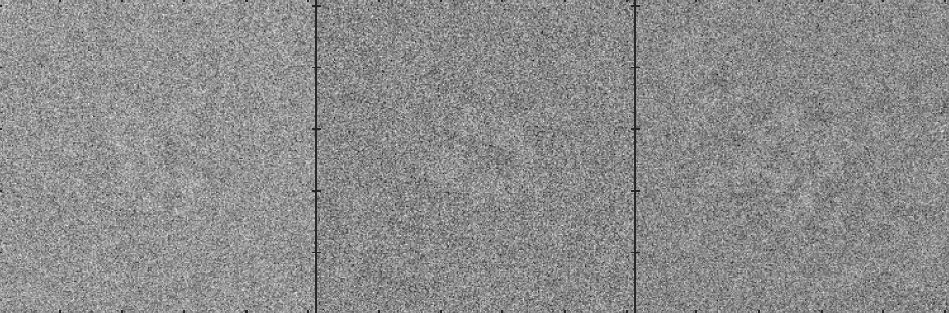
\includegraphics[width=.99\columnwidth]{figures/raw_expt_images.png}
\end{center}
\caption{Three raw cryo-EM images from an experimental dataset of TRPV1 \cite{trpv1_nature}}
\label{fig:raw_expt_images}
\end{figure}

\section{The Cryo-EM Revolution}
In 2015, cryo-EM was selected as the ``Method of the Year'' by the journal Nature Methods \cite{nature_method}. In the last five years, the Electron Microscopy Data Bank (EMDB) has been inundated with the deposition of high resolution structures. This wave of progress has been made possible by improved detector technology on one hand, along with better automation and software on the other. 

The ``goodness'' of a detector is captured by its detective quantum efficiency (DQE), which quantifies how much the signal to noise ratio (SNR) of the measurement is affected by the process of detection \cite{dainty1974}. The DQE ranges from 0 to 1, with 1 being characteristic of an ideal detector. Until recently, charge-coupled device (CCD) cameras were preferred for cryo-EM despite having a low DQE $\sim 0.1$ at high energies, due to the ease of automated data acquisition with them \cite{Sander200592}. In CCD cameras, the incident electrons are first converted into photons via a scintillator, a mechanism that is lossy and leads to further degradation of the already weak signal. Starting around 2012, a new generation of `direct electron detectors' spurred the onset of the current cryo-EM revolution \cite{faruki}. Direct electron detectors, as the name suggests, are able to detect electrons directly without first converting them to photons, resulting in a much higher DQE than CCD cameras. They also provide much faster readout, enabling collection of cryo-EM data in the `movie mode' in which several images are recorded in rapid succession. Electrons scattering from the cryo-EM sample cause movements of the sample leading to motion blur. With the captured movies, beam induced motion can now be tracked and corrected, facilitating de-blurring and retention of higher resolution information in images than before. Niko Grigorieff and his colleagues first demonstrated beam induced motion correction by leveraging the movie mode.

The improvement in detector technology was accompanied by new maximum likelihood based image analysis approaches, introduced by Fred Sigworth \cite{sigworth_rev} in 1998 \cite{sigworth1998}. The first notable results that heralded the cryo-EM revolution were from the University of California in San Francisco (UCSF), where a $3.3 \AA$ resolution map of the 20S proteasome was obtained using the K2 detector,and the Medical Research Council (MRC) in Cambridge, where ribosome structure details up to $4 \AA$ resolution were obtained from merely $35,000$ particle images from a Falcon detector \cite{ycheng_natmeth, Li2013InfluenceOE, Bai2013RibosomeST}. This was a significant milestone for cryo-EM from the $40 \AA$ structures in the early ``blog-ology'' era of the $1990$'s.

\section{Algorithmic Overview of Single Particle Reconstruction}

\begin{figure}[t]
\begin{center}
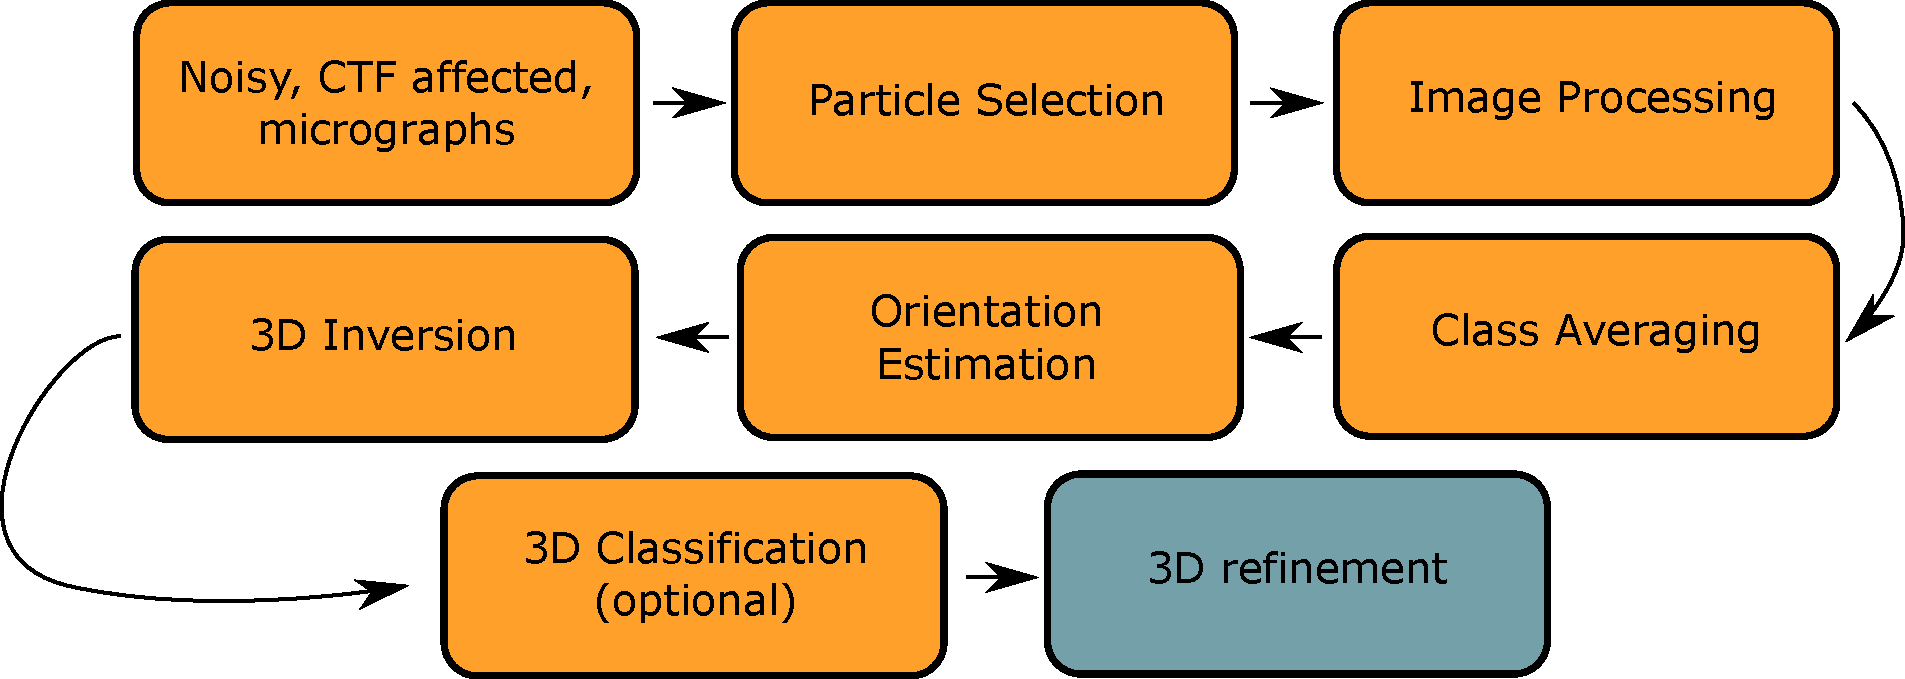
\includegraphics[width=.9\columnwidth]{figures/cryoem_full_pipeline.pdf}
\end{center}
\caption{Cryo-EM Pipeline}
\label{fig:cryoem_full_pipeline}
\end{figure}

The first step in SPR is collection of the data itself. The specimen frozen in an ice layer is imaged using an electron microscope. A top view  of the sample is acquired in the form of a large image called a micrograph. The subsequent steps of the SPR pipeline are as follows (see Fig. \ref{fig:cryoem_full_pipeline}):

\begin{itemize}
\item Particle Selection: Hundreds of thousands of individual particles need to be identified and picked from micrographs in the dataset, either semi-automatically or automatically. This step often needs manual intervention thereby making it time-consuming and prone to inconsistency \cite{Scheres2015SemiautomatedSO, Norousi2013AutomaticPU}. There have been many recent advancements to make particle selection fully automated, for instance, using deep learning and convolutional neural networks \cite{Wang2016DeepPickerAD}.

\item Image Preprocessing: Raw cryo-EM images are extremely noisy and suffer from additional effects of the contrast transfer function (CTF) of the microscope. Raw images are first preprocessed by whitening, normalization, denoising and other image processing techniques to prepare them for the next step.

\item Class Averaging or 2D Classification: Since cryo-EM images suffer from very low SNR's, neighboring images are first identified by partitioning the dataset using classification techniques. After alignment and averaging, the resulting images, called class averages, have a higher SNR and can be used for orientation estimation.

\item Orientation Estimation: Next, the viewing angles 
or pose parameters associated with the images are estimated using angular reconstitution or common-line based algorithms that leverage information in the common lines between pairs of images. This is possible due to the Fourier Projection Slice Theorem (see Appendix). Algorithms in the ASPIRE toolbox use convex optimization and spectral methods to achieve an orientation assignment that is as consistent as possible with all common lines.

\item 3D classification (optional): Cryo-EM images are often obtained from a heterogeneous mixture of a macromolecule in two or more of its conformations. It is thus important to reconstruct all possible 3D conformations from the images. This is called the `heterogeneity problem' in cryo-EM \cite{Katsevich2015CovarianceME, Tagare2015DirectlyRP}. 

\item 3D Inversion: Using classical tomography techniques, the 3D structure is reconstructed from 2D images whose orientations have been assigned.

\item Iterative Refinement: Using an ab-initio estimate as the starting 3D structure, the iterative refinement process uses the current estimate and the raw data to improve and refine the 3D structure until convergence.

\end{itemize} 
\subsection{Cryo-EM Software and Databases}
The EMDB, an archive for 3D EM reconstructions, now contains over $4000$ deposited maps, including several high resolution maps reflective of the ``resolution revolution''. In addition to final 3D structures, the need to publicly archive raw EM data for benchmarking and validation has been recognized by the cryo-EM community. The Electron Microscopy Public Image Archive (EMPIAR) is a repository dedicated to raw cryo-EM datasets. EMPIAR is designed to support large dataset transfer and contains terabytes of ``big data'' in the form of raw micrographs as well as movies.

There are many excellent open source software packages for structure reconstruction from cryo-EM images using statistical methods, such as RELION, SPIDER, Xmipp, FREALIGN, SPARX, EMAN2, SIMPLE, IMAGIC, etc. \cite{eman2, xmipp, spider, imagic, relion, frealign}. The algorithms in this dissertation are included and in the software toolbox ASPIRE, publicly available at \url{spr.math.princeton.edu}. 

SPR is a very challenging and computationally expensive inverse problem. The widespread accessibility of Graphical Processing Units (GPUs) in the recent years have vastly reduced the time needed to obtain 3D reconstructions from raw data \cite{gpurelion}.


\section{3D Ab-Initio and Homology Modeling}
The iterative refinement procedure in SPR requires an initial structure as the starting point. Starting from a good initial model can significantly reduce the number of iterations needed for convergence, and therefore lead to substantial savings in computational running time. Most refinement algorithms are based on some local optimization procedure, so there is no guarantee of converging to the global optimum solution. In particular, cryo-EM refinement suffers from the problem of 'model bias', meaning that the final solution is heavily influenced by the initial ab-initio model \cite{sigworth_rev}.

The quality of the initial model is less critical when the cryo-EM data itself enjoys a high SNR. In that case, relatively featureless initial models like ellipsoids can also converge to the global optimum using high quality data. However, in practice, the SNR is typically too low to allow this. For small complexes in particular, the images can be extremely noisy and refinement is challenging. There are a few approaches for determining a good ab-initio model to start the iterative refinement process. The method of moments and random conical tilt reconstruction provide low resolution ab-initio models \cite{Radermacher, Radermacher2, Salzman1990, Goncharov1986, Goncharov1988} . However, the method of moments is very sensitive to errors in the data and hence not very reliable in practice.

Yet another approach is based on common lines between images, also known as angular reconstitution. This is based on the observation that the common lines between three projection images uniquely determine their relative orientations up to chirality. There are several existing common lines based algorithms \cite{Penczek1996, farrow, mallick_cvpr, Singer2009, Shkolnisky2012ViewingDE}. In \cite{zhao}, the authors obtained ab-initio models for the E. coli 50S ribosomal subunit from 27,121 projection images and for the 70S ribosome from 40,779 projection images. With these models, the refinement process converged in one or two steps. However, all these algorithms require computation of class averages to improve the SNR of the images enough so that common lines based algorithms can succeed. It has not yet been possible to estimate 3D ab-initio models from raw images directly, without class averaging.

Our main motivation in this dissertation is to suggest algorithms for 3D homology modeling that do not require any class averaging, and that can succeed even for small complexes when images are very noisy. In this regime, other existing methods of refinement, class averaging, common lines approaches, fail. The suggested algorithms for 3D homology and ab-initio modeling in this dissertation are based on the theory developed by Zwi Kam \cite{kam1980}, and combine experimental design with innovative mathematical techniques. Kam showed in 1980 that the autocorrelation function of the 3D molecule over the rotation
group $SO(3)$ can be estimated from 2D projection images
whose viewing directions are uniformly distributed over the
sphere.

The main requirement for the success of these algorithms is for the number of images in the dataset to be large enough for PCA of the 2D projection images to give non-trivial eigenvalues, that is, a visible gap in the spectrum of the covariance matrix. Covariance estimation in the presence of noise and CTF's is a prerequisite to using Kam's method. In chapter 3, we first derive a new approach for covariance matrix estimation that takes the CTF and noise both into account.

Another requirement for Kam's theory to succeed is for the viewing angles of images to be uniformly distributed over the sphere. We investigate the effects of deviations from this in more detail in chapter 4.

In this dissertation, we focus on 3D ab-initio and homology modeling, and image restoration. In that spirit, we treat datasets as belonging to a single conformation (which is a good approximation when the dataset is largely homogeneous). In cases when the molecule may exhibit heterogeneity, that is the molecule can exist in two or more conformations, this  means obtaining its `average' 3D conformation. 

\section{Image Restoration}
Cryo-EM images suffer from degradation due to both electron noise and the effect of the microscope's point spread function, called the Contrast Transfer Function (CTF). The CTF is roughly a radially isotropic decaying sinusoid function in frequency space that is pointwise multiplied with the image in Fourier space. This results in inversion of the contrast where the CTF is negative, and complete loss of information at the `zero frequencies', which are the frequencies at which the CTF is zero. CTF correction is a challenging problem due to this non invertible nature of the CTF (see Fig.~\ref{fig:ctf_intro}). Phase flipping \cite{rev2} is a popular albeit sub-optimal technique that corrects only for the phases but not for the amplitudes of the Fourier coefficients. In phase flipping, the sign of Fourier coefficients is inverted at frequencies for which the CTF is negative. There exist other approaches such as classical Wiener filtering. Wiener filtering can be considered as careful division or inversion of the CTF operator so as to limit the accompanying noise amplification. Wiener filtering gives a linear estimate of the image that is optimal in terms of the mean squared error. In some approaches, CTF correction is handled much later in the cryo-EM pipeline at the 3D reconstruction stage \cite{Penczek_image, imagic, eman2, spider}. Cryo-EM micrographs are acquired at different microscope settings such as the defocus, so different images are affected by different CTF's. An optimal approach for CTF correction should correct for both the Fourier phases and amplitudes. This would require combining information from all images that are affected by different CTF's, to recover information lost at the zero crossings.

Image restoration in cryo-EM requires both denoising and CTF correction. Image restoration of the noisy, 2D projection images is required to aid the process of 3D reconstruction itself. Typically, 3D reconstruction is performed starting from class averages which enjoy a higher SNR than raw images. There are several methods to decrease the noise level using low pass filters, wavelet transforms, non-local mean filters, bilateral filters, etc. \cite{Wang2013AZN, Jiang2003ApplicationsOA, Sorzano2006ImprovedBI, Wei2010211}. The main challenge in denoising is to retain important features in the image while reducing the noise.

\begin{figure}
\begin{center}
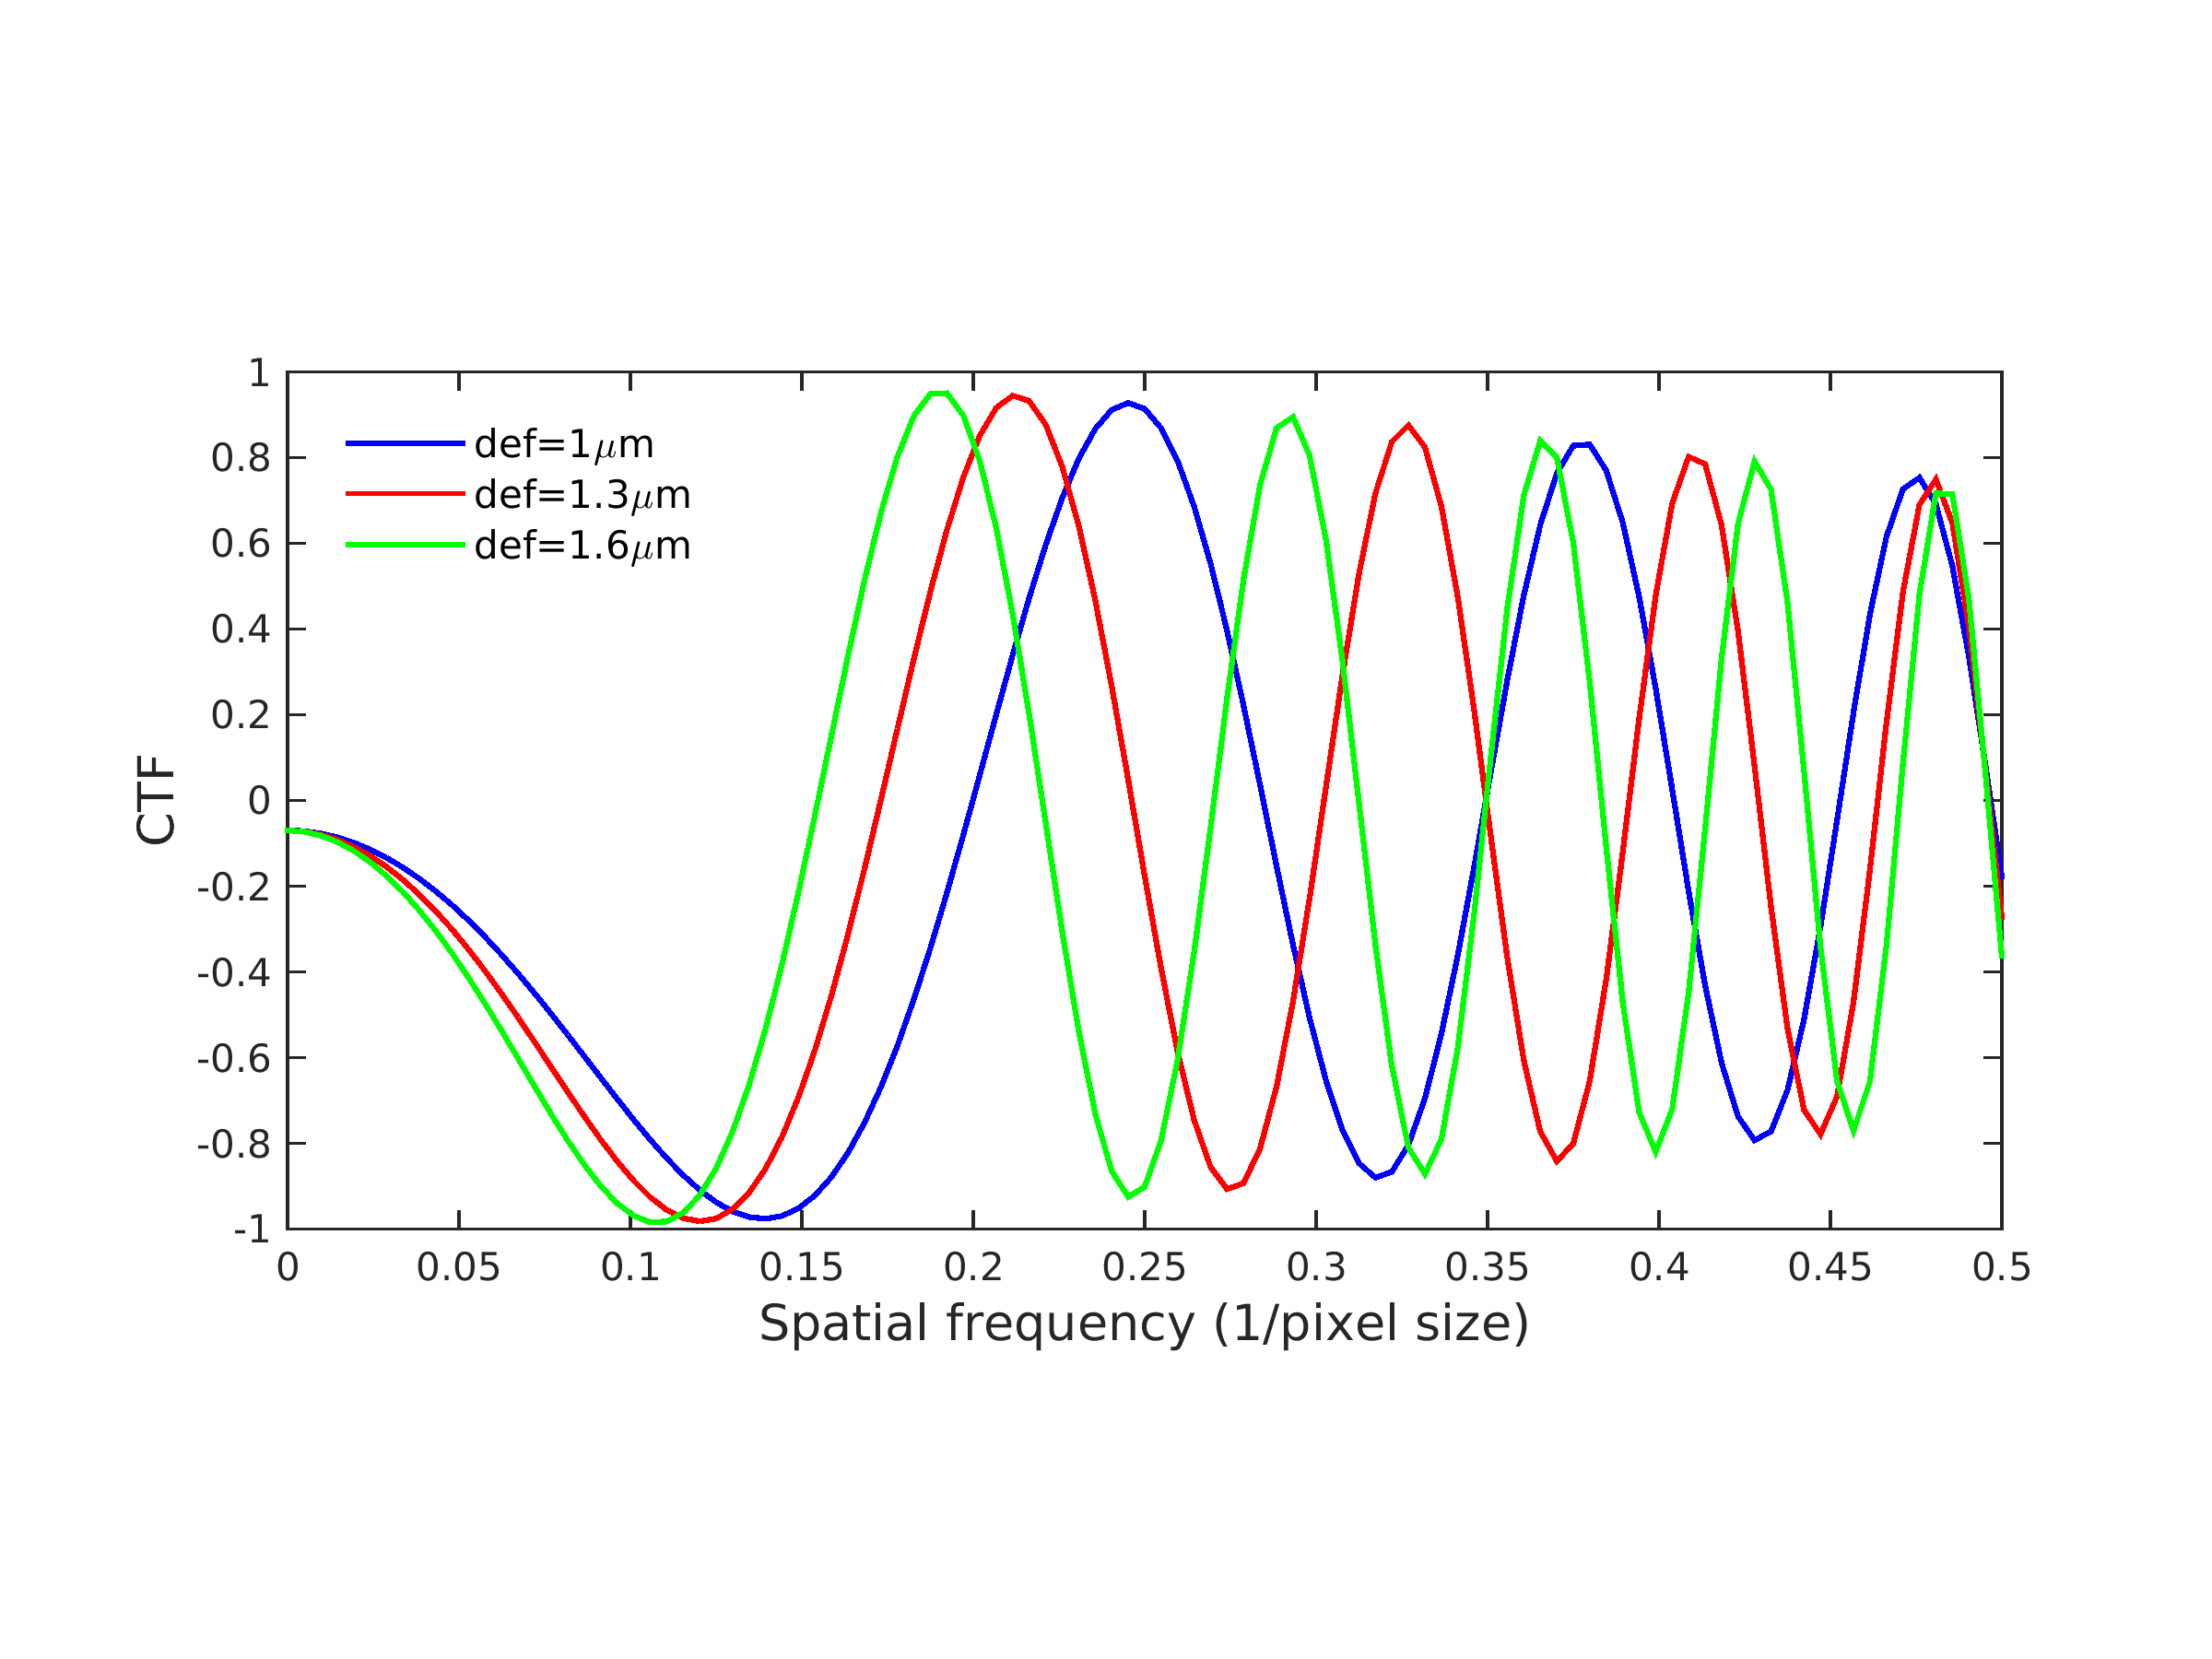
\includegraphics[width=.99\columnwidth]{figures/ctfeg_fig.png}
\caption{CTF's for different values of the defocus. CTF parameters used are: the amplitude contrast $\alpha = 0.07$
, the electron wavelength $\lambda= 2.51pm$, the spherical aberration constant $Cs=2.0$
, the B-factor $B=10$, the defocus$=1\mu m, 1.3\mu m,$ and
$1.6\mu m$, and the pixel size is $2.82\AA$.}\label{fig:ctf_intro}
\end{center}
\end{figure}


\section{Contributions}
In this thesis, we introduce new algorithms for 3D homology and ab-initio modeling in cryo-EM, that leverage Kam's theory and generalize the molecular replacement method in X-ray crystallography. We foresee these new algorithms to enable reconstruction of small complexes for which existing methods of refinement, class averaging and common-lines approaches fail because the images are very noisy. Our algorithms combine mathematical innovation with experimental design, and are less restrictive in terms of the SNR required for other approaches to succeed. 

In Chapter 1, we introduce two new algorithms for homology and ab-initio modeling based on Kam's theory. The autocorrelation function determines the expansion coefficients of the 3D molecule in spherical harmonics up to an orthogonal matrix of size $(2l+1)\times (2l+1)$ for each $l=0,1,2,\cdots$. In this chapter we show how techniques for solving the phase retrieval problem in X-ray crystallography can be modified for the cryo-EM setup for retrieving the missing orthogonal matrices. Specifically, we present two new approaches that we term {\em Orthogonal Extension} and {\em Orthogonal Replacement}, in which the main algorithmic components are the singular value decomposition and semidefinite programming. We demonstrate the utility of these approaches through numerical experiments on simulated data.

Our homology and ab-initio modeling approaches require an estimator for the covariance matrix of the underlying clean images. The covariance estimator can be leveraged for image restoration. The problem of image restoration in cryo-EM entails correcting for the effects of the Contrast Transfer
Function (CTF) and noise. Popular methods for image restoration include
`phase flipping', which corrects only for the Fourier phases but not amplitudes, and Wiener filtering, which
requires the spectral signal to noise ratio. In chapter 3, we propose a new image restoration method
which we call `Covariance Wiener Filtering' (CWF).
In CWF, the covariance matrix of the projection images is used within the 
classical Wiener filtering framework for solving the image restoration 
deconvolution problem. Our estimation procedure for the covariance matrix is new 
and successfully corrects for the CTF.   
We demonstrate the efficacy of CWF by applying it to restore both simulated and experimental cryo-EM images.
Results with experimental datasets demonstrate that CWF provides a good way to 
evaluate the particle images and to see what the dataset contains even without 2D 
classification and averaging.

One of the main challenges in cryo-EM is the typically low signal to noise ratio (SNR) of the acquired images. 2D classification of images, followed by class averaging, improves the SNR of the resulting averages, and is used for selecting particles from micrographs and for inspecting the particle images. In chapter 4, we introduce a new affinity measure, akin to the Mahalanobis distance, to compare cryo-EM images belonging to different defocus groups. The new similarity measure is employed to detect similar images, thereby leading to an improved algorithm for class averaging. We evaluate the performance of the proposed class averaging procedure on synthetic datasets, obtaining state of the art classification. 

Finally, in chapter 5, we utilize the covariance matrix estimator from CWF and integrate it into the Orthogonal Retrieval procedure.
The missing phase problem in X-ray crystallography is commonly solved using the
technique of molecular replacement \cite{rossmann62, rossmann01, scapin13}, 
which borrows phases from a previously
solved homologous structure, and appends them to the measured Fourier magnitudes
of the diffraction patterns of the unknown structure. More recently, molecular 
replacement has been proposed for solving the missing orthogonal matrices 
problem arising in Kam's autocorrelation analysis \cite{kam1977, kam1980} for 
single particle reconstruction using X-ray free electron lasers 
\cite{Saldin2009, Hosseinizadeh2015, Starodub12ncom} and cryo-EM \cite{Bhamre2014}. In classical
molecular replacement, it is common to estimate the magnitudes of the unknown 
structure as twice the measured magnitudes minus the magnitudes of
the homologous structure, a procedure known as 
`twicing' \cite{tukey77}. Mathematically, this is equivalent to finding an 
unbiased estimator for
a complex-valued scalar \cite{Main1979}. We generalize this scheme for the
case of estimating real or complex valued matrices arising in single particle 
autocorrelation analysis. We name this approach ``Anisotropic Twicing'' 
because unlike the scalar case, the unbiased estimator is not obtained by a 
simple magnitude isotropic correction. We compare the performance of the least 
squares, twicing and anisotropic twicing estimators on synthetic and 
experimental datasets. We demonstrate 3D homology modeling in cryo-EM directly from experimental data without iterative refinement or class averaging, for the first time.
